\subsection{Facilities Status}
\label{Sec:Facilities}
Collisions of heavy nuclei at ultra-relativistic energies are studied at two facilities: the Relativistic Heavy Ion Collider (RHIC) at Brookhaven National Laboratory, and (since 2010) the Large Hadron Collider (LHC) in Geneva, Switzerland. The impressive experimental progress in the field since the 2007 Long Range Plan that is presented in what follows has been made possible by the outstanding performance of these two facilities. 

RHIC began operations in 2000 with the capability of colliding nuclei from deuterons to Au at center-of-mass energies of 
200 GeV per nucleon pair.\footnote{RHIC also can collide  polarized protons at energies up to $\sqrt{s}=510$~GeV. This unique capability forms the basis of the RHIC Spin program\cite{Aschenauer:2015eha} discussed in the Cold QCD Town Meeting White Paper.}
Recommendation IV of the 2007 Long Range Plan endorsed the ``RHIC II'' luminosity upgrade, envisioned as a 10-20 fold increase above the design luminosity of $2 \times 10^{26}\ \mathrm{cm^{-2} s^{-1}}$ for full energy \AuAu\ collisions. 
While this upgrade was a high priority of the nuclear science community, the then-estimated cost of $\sim$\$150M drove a proposed funding profile that would have provided this capability no earlier than 2016. Remarkably, breakthroughs in both transverse and longitudinal stochastic cooling by the BNL Collider-Accelerator Department scientists have made it possible to achieve luminosities well above the RHIC II specification 3 years earlier at roughly 15\% of the cost projected in 2007. The new RHIC luminosity performance is shown in the left panel of Figure~\ref{Fig:RHICLum},
demonstrating that the \AuAu\ luminosity from the 2014 RHIC run routinely exceeded RHIC II luminosities. As a result, the integrated luminosity for \AuAu\ collisions acquired in Run 14 significantly exceeds the sum of {\em all} previous RHIC runs\cite{RHICPerformance}, as shown in the right panel of Figure~\ref{Fig:RHICLum}.
\begin{figure}[ht]
\centerline{
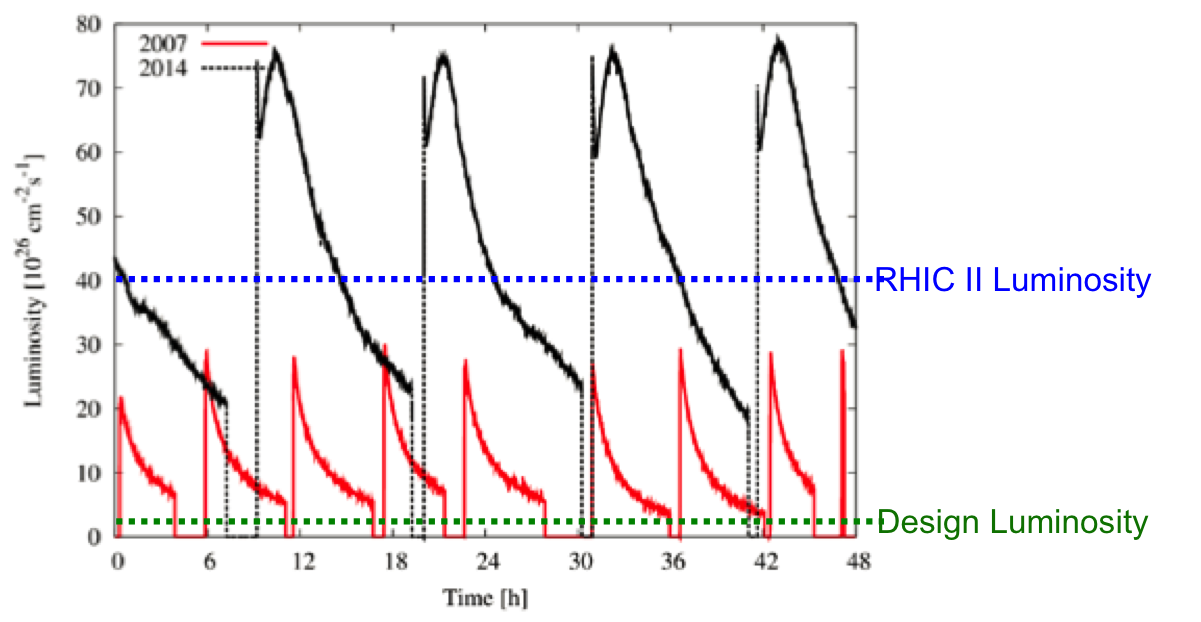
\includegraphics[width=0.60\textwidth]{fig/RHICLuminosity.png}
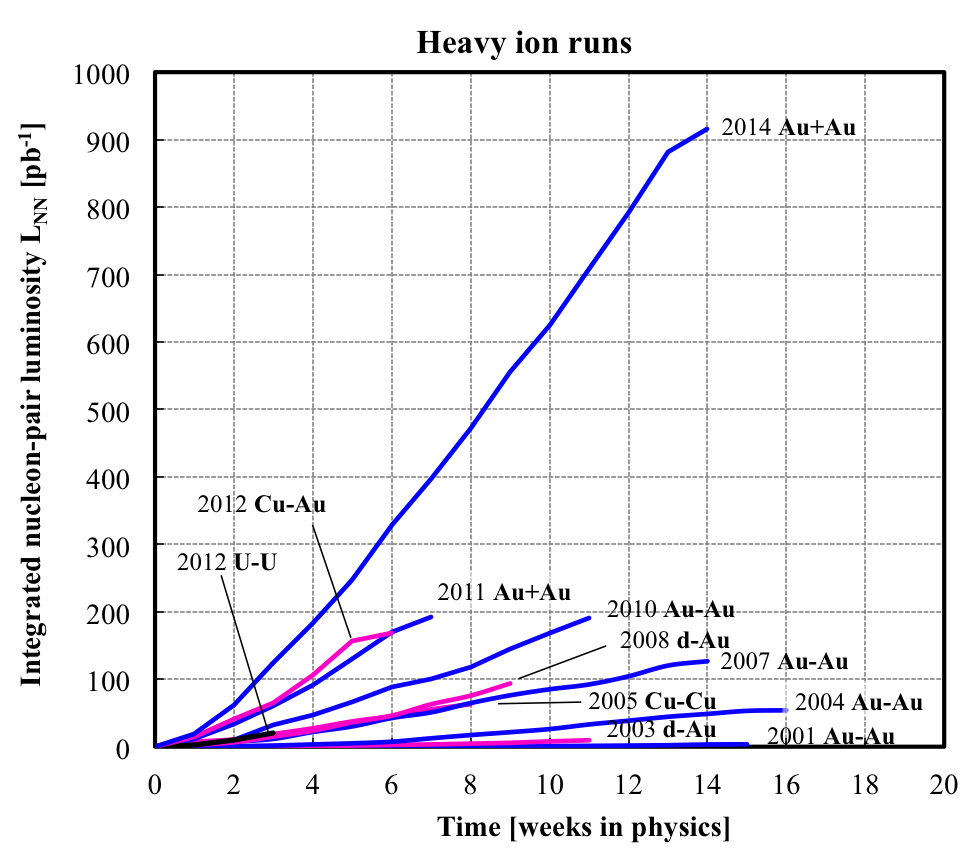
\includegraphics[width=0.40\textwidth]{fig/RhicIntegratedLuminosityAA.png}
}
\caption[RHIC luminosity, past and present]{Left: the luminosity for $\sqrt{s_{NN}}=200$~GeV \AuAu\ collisions as a function of time in the 2014 RHIC Run, compared to RHIC and RHIC II design luminosity.
Right: the integrated luminosity for all RHIC heavy ions runs.
}
\label{Fig:RHICLum}
\end{figure}

RHIC's capabilities were extended in 2011 with the commissioning 
of an Electron Beam Ion Source\cite{Alessi:2010zz} 
(EBIS)\footnote{EBIS was partially funded by NASA for the study of space radiation effects on extended human space missions
at NASA's Space Radiation Laboratory located at BNL.}, 
which replaced the aging Tandem Accelerator as a source for injection into the AGS/RHIC accelerator chain. The new physics enabled by EBIS was demonstrated in definitive fashion in 2012, when RHIC became the first collider to produce \UU\ collisions. 
The intrinsic deformation of the ${}^{238}$U nucleus provides a valuable tool 
in constraining models of the initial state energy deposition 
and separating the effects from overlap geometry and quantum fluctuations in the initial state on the hydrodynamic flow in the final state.
Similarly, in 2014 RHIC provided the first \HeAu\ collisions to study the development of odd-harmonic hydrodynamic flow resulting from the three nucleons in ${}^3$He. Both of these developments are described in more detail in Section~\ref{Sec:Flow}.

Another demonstration of the flexibility of the RHIC is the Beam Energy Scan (BES) in search of the QCD critical point.  Phase I of this campaign was conducted in 2010, 2011 and 2014. In addition to full energy \AuAu\ collisions at $\sqrt{s_{NN}} = 200$~GeV, data were taken for \AuAu\ collisions at 
$\sqrt{s_{NN}}$ 62.4 GeV, 39 GeV, 27 GeV, 19.6 GeV, 14.5 GeV, 11.5 GeV and 7.7 GeV. As discussed in more detail in Section~\ref{Sec:BES} this range of energies explores the region in the QCD phase diagram (as a function of baryon chemical potential $\mu_B$ and temperature) in which it is predicted that the smooth cross-over transition observed at the highest RHIC energies transforms into a first-order phase transition. The capability to explore this regime is a unique feature of RHIC.

Both the PHENIX\cite{PHENIX} and the STAR\cite{STAR} experiments at RHIC have undergone significant upgrades since the last Long Range Plan. PHENIX extended its measurement capabilities at forward angles with a Muon Piston Calorimeter\cite{Chiu:2007zy}, which is now being upgraded with a pre-shower detector\cite{Campbell:2013zw}. 
STAR increased its data acquisition and triggering capabilities via the DAQ1000\cite{STAR:DAQ1000} and High Level Trigger\cite{STAR:HLT}
projects. The Time of Flight\cite{STAR:TOF} detector greatly extended their particle identification capabilities
and together with the muon telescope  detector\cite{Ruan:2009ug} significantly improved its capabilities to study physics in the di-lepton channel.
Both experiments installed silicon-based tracking systems for vertexing and heavy-flavor detection, 
the VTX\cite{Nouicer:2008pf,Taketani:2010zz} and FVTX\cite{Aidala:2013vna} for PHENIX and the HFT\cite{Kapitan:2008kk,Qiu:2014dha} for STAR. These new capabilities, together with the greatly increased RHIC luminosity, are the realization of the RHIC II upgrade envisioned in the 2007 Long Range Plan.

\begin{figure}[!htb]
\begin{center}
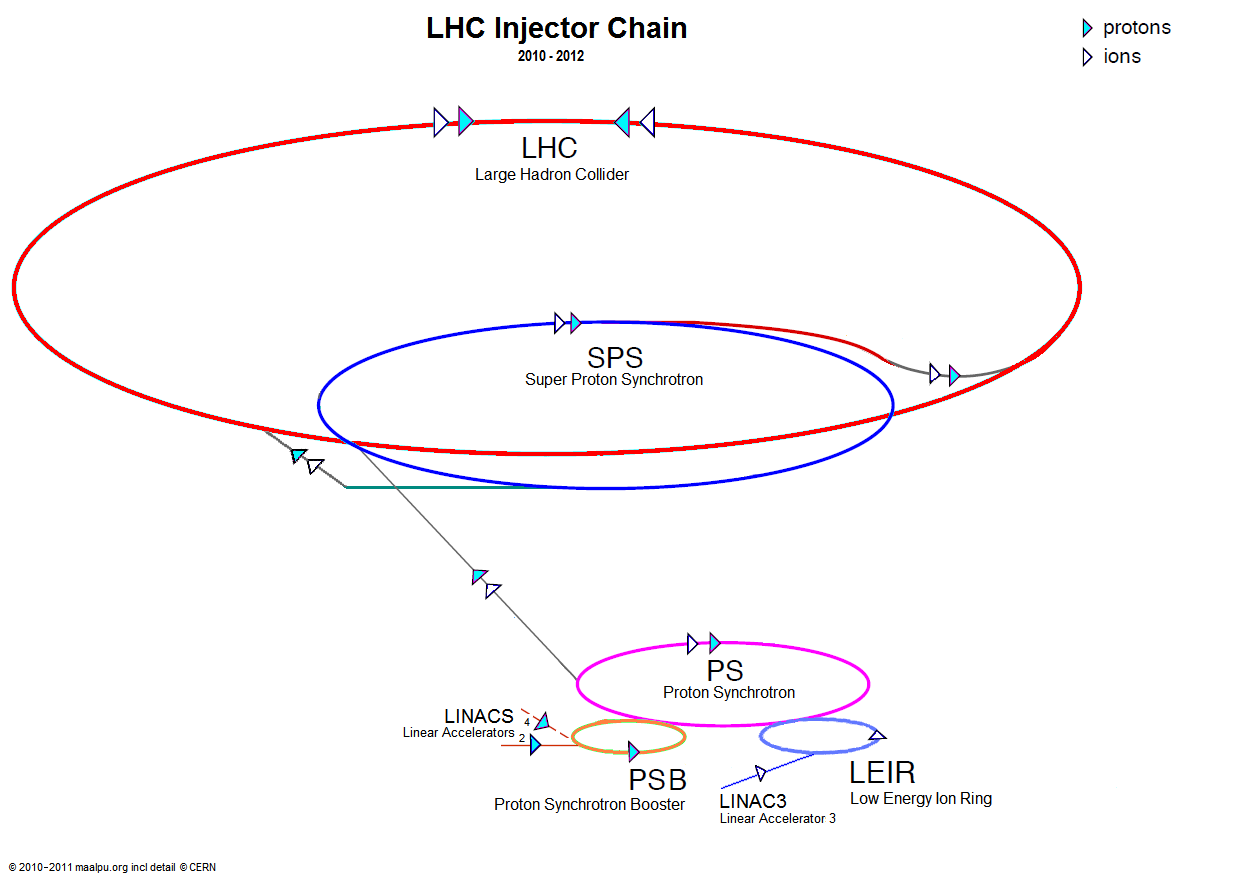
\includegraphics[width=0.8\textwidth]{fig/LHC_chain.png}
\caption{Schematic view of the LHC accelerator complex}
\label{fig:lhc_complex}
\end{center}
\end{figure}
 
Late 2009 marked the beginning of CERN LHC operations, with a pilot run providing
first proton+proton collisions with collision energies of 0.9 and 2.36~TeV. 
The first year of LHC physics running began with p+p running at 7~TeV in April 2010 and 
ended with first Pb+Pb collisions at $\rootsNN = 2.76$~TeV in November and 
December, increasing the center-of-mass energy explored in heavy ion collisions by a factor 
of 14 compared to RHIC. The heavy ion program, which was foreseen in LHC
planning from the beginning, uses most of the elements of the LHC 
accelerator chain shown in in Figure~\ref{fig:lhc_complex}, beginning
from the electron cyclotron resonance ion source and linear accelerator, 
which provide $^{208}$Pb ions stripped to Pb$^{29+}$ at 4.2 MeV/n.
After further carbon foil stripping, bunch shaping and 
electron cooling in the CERN Low Energy Ion Ring (LEIR),  
Pb$^{54+}$ ion bunches are sent to the CERN PS, accelerated and fully stripped,
yielding Pb$^{82+}$.  After acceleration in the SPS to to 177 GeV/n,
injection and acceleration in the LHC are the final steps. 
Using 120 colliding bunches for each beam, a peak luminosity of 
$3 \times 10^{25} \mathrm{cm}^{-2} \mathrm{s}^{-1}$ was achieved 
in the 2010 LHC run.  This corresponds to an 
integrated luminosity of 7~$\mu \mathrm{b}^{-1}$ delivered to each
of three interaction regions for the ALICE, ATLAS and CMS experiments
participating in heavy-ion data taking. 

\begin{figure}[ht]
\centerline{
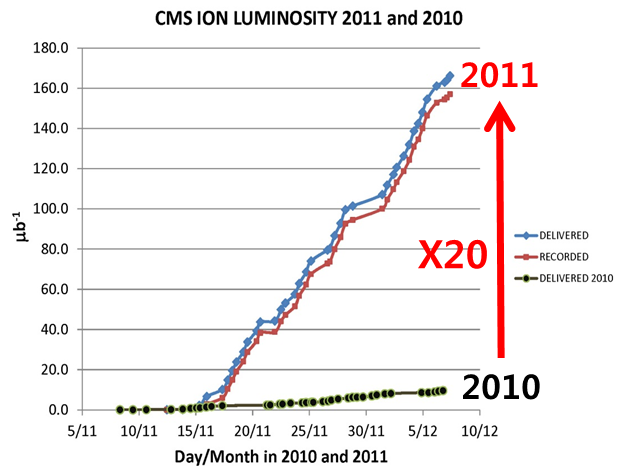
\includegraphics[width=0.55\textwidth]{fig/IntegratedLumPbPb.png}
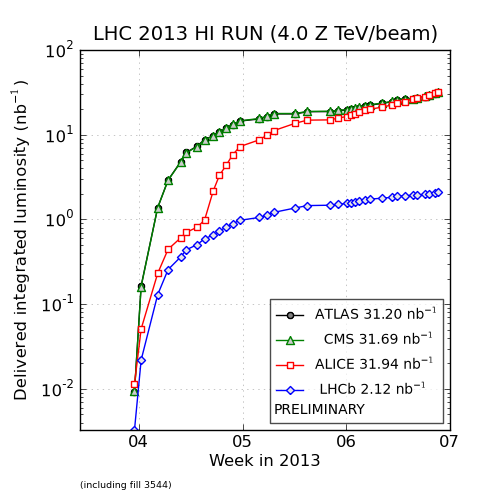
\includegraphics[width=0.45\textwidth]{fig/IntegratedLumpPbII.png}
}
\caption[LHC luminosity]{Left: Delivered and recorded integrated luminosities at 
CMS for $\sqrt{s_{NN}}=2.76$~GeV \PbPb\ collisions as a function of 
time for the 2010 and 2011 LHC Pb+Pb runs.
Right: Integrated luminosity for the $\sqrt{s_{NN}}=5.02$~TeV p+Pb 2013 LHC Run.
}
\label{Fig:LHCLum}
\end{figure}
For the November--December 2011 run, an increase in the number of 
colliding bunches to 360 per ring, as well as improved focusing, allowed 
an increase in peak luminosity by a factor of 15--20, reaching close to 
design collision rates. The total delivered luminosity per interaction region 
was about 150~$\mu \mathrm{b}^{-1}$, with delivered and 
recorded luminosity in CMS shown in Figure~\ref{Fig:LHCLum} (left).

The third heavy-ion data taking period in early 2013 provided proton+lead and lead+proton
collisions at 5.02~TeV, following a pilot run in fall 2012.
Although this mode of operation was not foreseen in the baseline design of the LHC,
beams were commissioned in 10 days. The physics requirements of all experiments 
were met in three weeks of physics running, resulting in an integrated luminosity of up to 
35~$n \mathrm{b}^{-1}$ and record intensity levels, Figure~\ref{Fig:LHCLum} (right).  
A p+p reference data set at 2.76~TeV was also recorded. 

All four major LHC detectors have participated in heavy-ion data taking
in the 2009--2013 period (Run I), with ALICE, ATLAS and CMS taking p+p, p+Pb and
Pb+Pb data, and LHCb taking p+p and p+Pb data. ALICE\cite{ALICE} has been optimized
for heavy-ion operations, with large kinematic coverage, in particular at low 
transverse momenta, and charged particle identification over a wide 
momentum range using a variety of techniques. ATLAS\cite{ATLAS} and CMS\cite{CMS} are general purpose
collider detectors, with a particular focus on high data taking rates, full 
azimuthal coverage over a wide rapidity range and high resolution at very 
high transverse momenta. Although designed for discovery physics in p+p 
collisions, the high granularity of ATLAS and CMS makes them suitable
for heavy-ion collisions as well, in particular for high momentum 
probes where they complement the strengths of the ALICE detector. The heavy-ion 
related program of LHCb\cite{LHCb} was focussed on quarkonia measurements in p+Pb 
collisions at forward rapidities.